\hypertarget{preface}{%
\section*{Preface}\label{preface}}

\hypertarget{i-aim-of-the-specification}{%
\subsection*{I. Aim of the
Specification}\label{i-aim-of-the-specification}}

This document is one of several related specifications which aim to
provide a common set of usage descriptions of international standards
for packaging digital information for archiving purposes. These
specifications are based on common, international standards for
transmitting, describing and preserving digital data. They also utilise
the Reference Model for an Open Archival Information System (OAIS),
which has Information Packages as its foundation. Familiarity with the
core functional entities of OAIS is a prerequisite for understanding the
specifications.

The specifications are designed to help data creators, software
developers, and digital archives to tackle the challenge of short-,
medium- and long-term data management and reuse in a sustainable,
authentic, cost-efficient, manageable and interoperable way. A
visualisation of the current specification network can be seen here:

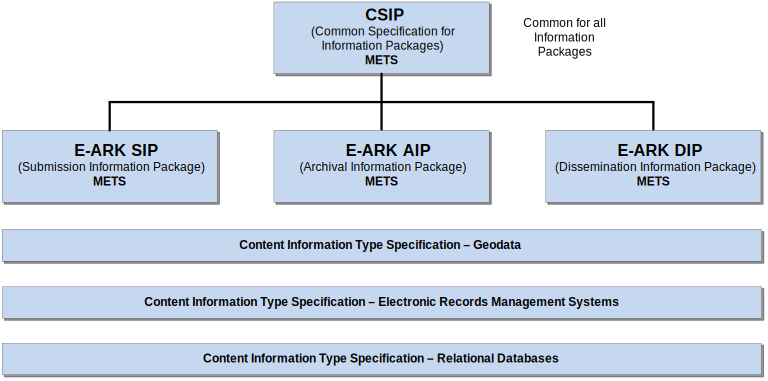
\includegraphics{figs/fig_1_dip.png}

\textbf{Figure I:} Diagram showing E-ARK specification dependency
hierarchy. Note that the image only shows a selection of the published
CITS and isn't an exhaustive list.

\hypertarget{overview-of-the-e-ark-specifications}{%
\subsubsection*{Overview of the E-ARK
Specifications}\label{overview-of-the-e-ark-specifications}}

\hypertarget{common-specification-for-information-packages-e-ark-csip}{%
\paragraph{Common Specification for Information Packages (E-ARK
CSIP)}\label{common-specification-for-information-packages-e-ark-csip}}

This document introduces the concept of a Common Specification for
Information Packages (CSIP). The main purposes of CSIP are to:

\begin{itemize}
\tightlist
\item
  Establish a common understanding of the requirements which need to be
  met to achieve interoperability of Information Packages.
\item
  Establish a common base for the development of more specific
  Information Package definitions and tools within the digital
  preservation community.
\item
  Propose the details of an XML-based implementation of the requirements
  using, to the largest possible extent, standards which are widely used
  in international digital preservation.
\end{itemize}

Ultimately the goal of the Common Specification is to reach a level of
interoperability between all Information Packages so that tools
implementing the Common Specification can be adopted by institutions
without the need for further modifications or adaptations.

\hypertarget{specification-for-submission-information-packages-e-ark-sip}{%
\paragraph{Specification for Submission Information Packages (E-ARK
SIP)}\label{specification-for-submission-information-packages-e-ark-sip}}

The main aims of this specification are to:

\begin{itemize}
\tightlist
\item
  Define a general structure for a Submission Information Package format
  suitable for a wide variety of archival scenarios, such as document
  and image collections, databases or geospatial data.
\item
  Enhance interoperability between Producers and Archives.
\item
  Recommend best practices regarding the structure, content and metadata
  of Submission Information Packages.
\end{itemize}

\hypertarget{specification-for-archival-information-packages-e-ark-aip}{%
\paragraph{Specification for Archival Information Packages (E-ARK
AIP)}\label{specification-for-archival-information-packages-e-ark-aip}}

The main aims of this specification are to:

\begin{itemize}
\tightlist
\item
  Define a generic structure of the AIP format suitable for a wide
  variety of data types, such as document and image collections,
  archival records, databases or geospatial data.
\item
  Recommend a set of metadata related to the structural and the
  preservation aspects of the AIP as implemented by the eArchiving
  Reference Implementation (earkweb).
\item
  Ensure the format is suitable to store large quantities of data.
\end{itemize}

\hypertarget{specification-for-dissemination-information-packages-e-ark-dip}{%
\paragraph{Specification for Dissemination Information Packages (E-ARK
DIP)}\label{specification-for-dissemination-information-packages-e-ark-dip}}

The main aims of this specification are to:

\begin{itemize}
\tightlist
\item
  Define a generic structure of the DIP format suitable for a wide
  variety of archival records, such as document and image collections,
  databases or geographical data.
\item
  Recommend a set of metadata related to the structural and access
  aspects of the DIP.
\end{itemize}

\hypertarget{content-information-type-specifications-e-ark-cits}{%
\paragraph{Content Information Type Specifications (E-ARK
CITS)}\label{content-information-type-specifications-e-ark-cits}}

The main aim of a Content Information Type Specification (CITS) is to:

\begin{itemize}
\tightlist
\item
  Define, in technical terms, how data and metadata must be formatted
  and placed within a CSIP Information Package to achieve
  interoperability in exchanging specific Content Information.
\end{itemize}

The number of possible Content Information Type Specifications is
unlimited. For a list of existing Content Information Type
Specifications see the DILCIS Board webpage (DILCIS Board,
\href{http://dilcis.eu/}{http://dilcis.eu/}).

\hypertarget{ii-organisational-support}{%
\subsection*{II. Organisational
Support}\label{ii-organisational-support}}

This specification is maintained by the Digital Information LifeCycle
Interoperability Standards Board (DILCIS Board,
\href{http://dilcis.eu/}{http://dilcis.eu/}). The role of the DILCIS
Board is to enhance and maintain the draft specifications developed in
the European Archival Records and Knowledge Preservation Project (E-ARK
project, \href{http://eark-project.com/}{http://eark-project.com/}),
which concluded in January 2017. The Board consists of eight members,
but no restriction is placed on the number of participants taking part
in the work. All Board documents and specifications are stored in GitHub
(\href{https://github.com/DILCISBoard/}{https://github.com/DILCISBoard/}),
while published versions are made available on the Board webpage. The
DILCIS Board have been responsible for providing the core specifications
to the Connecting Europe Facility eArchiving Building Block
\href{https://ec.europa.eu/cefdigital/wiki/display/CEFDIGITAL/eArchiving/}{https://ec.europa.eu/cefdigital/wiki/display/CEFDIGITAL/eArchiving/}.

\hypertarget{iii-authors--revision-history}{%
\subsection*{III. Authors \& Revision
History}\label{iii-authors--revision-history}}

A full list of contributors to this specification, as well as the
revision history, can be found in the
\protect\hyperlink{postface}{Postface material}.
